\documentclass{article}
\usepackage[T1]{fontenc}
\usepackage[utf8]{inputenc}
\usepackage[a4paper, total={6in, 8in}]{geometry}
%\usepackage[icelandic]{babel}
\usepackage{graphicx} %package to manage images

\usepackage{hyperref}
\usepackage{siunitx}
\usepackage{tabularx}

\usepackage{xcolor}
\usepackage{listings}

\colorlet{mygray}{black!30}
\colorlet{mygreen}{green!60!blue}
\colorlet{mymauve}{red!60!blue}

\lstset{
  backgroundcolor=\color{gray!10},  
  basicstyle=\ttfamily,
  columns=fullflexible,
  breakatwhitespace=false,      
  breaklines=true,                
  captionpos=b,                    
  commentstyle=\color{mygreen}, 
  extendedchars=true,              
  frame=single,                   
  keepspaces=true,             
  keywordstyle=\color{blue},      
  language=c++,                 
  numbers=none,                
  numbersep=5pt,                   
  numberstyle=\tiny\color{blue}, 
  rulecolor=\color{mygray},        
  showspaces=false,               
  showtabs=false,                 
  stepnumber=5,                  
  stringstyle=\color{mymauve},    
  tabsize=3,                                     
  title=\lstname 
}

\title{Embedded Group Project\\ \large Project 2 - Speed Controller}

\author{Steinarr Hrafn Höskuldsson\\
Arnþór Gíslason\\
Andrew Madden\\
\\
Reykjavik University}
\date{September 2022}


\newcommand{\mycomment}[1]{}
\newcommand{\timerinterval}{5ms }

\begin{document}
\maketitle
 % how to comment, input image and code
\mycomment{
\begin{figure}[h]
    \centering
    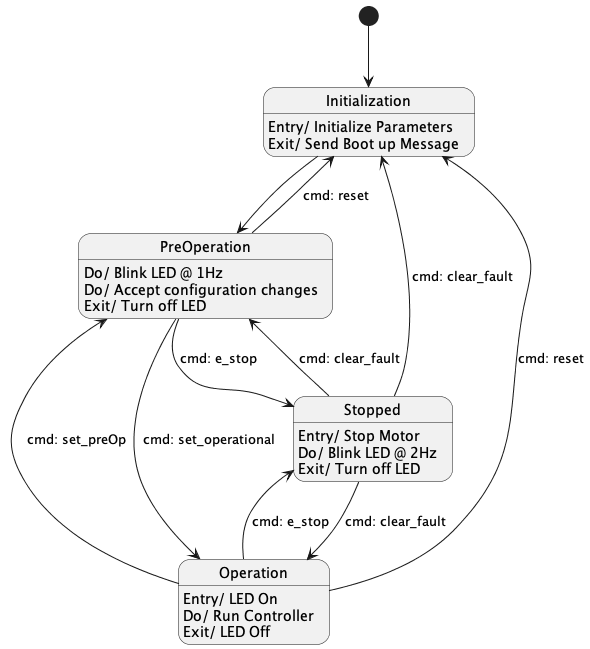
\includegraphics[width=0.75\textwidth]{Project3ControllerStateMachine/out/Project3ControllerStateMachine/docs/uml/uml.png}
    \caption{UML}
    \label{fig:UML}
\end{figure}

\lstinputlisting[caption=Defining 'ColorMatch' state, label={lst:colormatch}, language=Python, firstline=44, lastline=52]{LAB3/Basic.py}

}

\section{Part 1}
\begin{quote}
    
Implement the Initialization and Operational states and the reset command.  You can use the Arduino Serial class to issue simple commands from the keyboard to trigger a state transition.
\end{quote}

A communication scheme was devised. To send a command, e.g. an order to switch between states, only a single upper case letter should be sent. To set a variable a string on the form '(lower case letter)=(floating point value)' shall be sent, the letter indicates which value to be set. Things sent can not be longer than 10 characters and should be separated by a newline character.
\\
Functions to receive Serial input were added to our \verb!HackySerial! module. A function was written that parses a string on the form: \verb!p=3.45! to a "\verb!Parsed!" struct, which contains the character, 'p' and the floating point number 3.45.
\\
A program was written based on Refactoring Guru's state machine example. In the main loop a section was written that asynchronously receives data on the Serial port according to the communication scheme and switches between states on appropriate commands.

A lot of work was put into moving the programming of each state into it's own file. However that work was concurrent with the debugging of the control code and we ran out of time and were unable to merge the divergent branches.

A state diagram was created using PlantUML. The State Diagram can be seen in Figure \ref{fig:UML}

\begin{figure}[H]
    \centering
    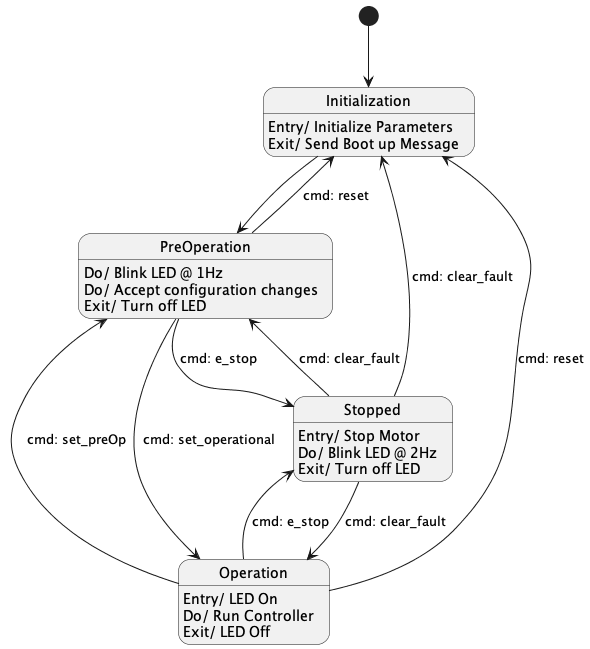
\includegraphics[width=0.75\textwidth]{Project3ControllerStateMachine/out/Project3ControllerStateMachine/docs/uml/uml.png}
    \caption{UML}
    \label{fig:UML}
\end{figure}

\section{Part 2}


Brake was implemented in the \verb!motor_controller! class where two methods were tried. First method was setting the set point to 0 and have the motor controller apply active breaking and second method was using the h bridge to short the poles of the motors effectively providing passive brake. 
\\
For this application, having active brakes wasn't needed to stop the motor in a suitable time and there wasn't any active load on the system which could've caused the motor to creep forwards. Adding active braking would also have introduced complexity in the program which might cause safety issues.

\section{Part 3}

\subsection{PI\_controller}
Instead of having \verb!PI_controller! inherit from \verb!P_controller! a new base class, \verb!controller! , was made that housed the common variables. Update was then implemented in \verb!PI_controller! and \verb!P_controller!. Alternatively, \verb!PI_controller! could've inherited from \verb!PI_controller! and overridden update().
\\
The \verb!PI_controller! subsists of both proportional gain and integral gain where the proportional gain is the error between set point and actual multiplied by an adjustable scalar, and the integral gain is the accumulated error over time.
\\
In order to overcome losses in a system, integral gain is a vital factor of the control system. In the case where there's no integral factor, the controller will not reach the desired set point and any attempts to reach the desired set point by increasing the proportional gain will result in the system becoming unstable.
\\
With an integral factor the accumulated error will result in an ever increasing output until the actual value reaches the set point and the integral starts to become stable.

\subsubsection{Windup Guard}

When the actual value either takes too long to reach the setpoint or the load on the system is enough to prevent the motor from reaching the set point a condition may arise where the integral grows excessively large and it may take the system some time to wind the integral down. A simple method  to prevent this condition is to limit the internal integral value to not exceed the output limits.

\subsection{RPM Gauge}

The first iteration of the rpm metering module consisted of a timer running at a set period, \verb!delta_t!, and each cycle the interrupts were counted between cycles. This method resulted in a fairly accurate value that was mostly immune to inaccuracies in the encoder wheel. However, the resolution of the measured rpm was around 400rpm,it was deemed too inaccurate and a new method was implemented.
\\
With the new method, a counter was set up that incremented at $500ns$ intervals and instead of counting the amount of interrupts during a set period the time between pulses was measured. When the timer overflows it's safe to assume that the motor is stationary and rpm is zero. 
\[ rpm=\frac{60\cdot} {PPR} \cdot t\]
Where 60 is seconds to a minute, ppr is pulses per revolution and t is time it took between pulses. 
\\
Absolute time can be found with \(t = \frac{t_c}{counts}\)  where $t_c$ is time/count and counts is ultimate count between pulses 
\\
At first, both phases of the encoder were used but what's believed to be inaccuracies in the positioning of the sensors of the encoder resulted in the measured value jumping 1000rpm often during the revolution, hardly any better than the previous method.
\\
After changing to using a single phase of the encoder, the measured value reached acceptable repeatability, however, a repeating pattern may be seen in the waveform which is  likely attributed to manufacturing tolerances in the magnetic encoder wheel. See \ref{fig:distortedRpm}.

\begin{figure}[h!t]
    \centering
    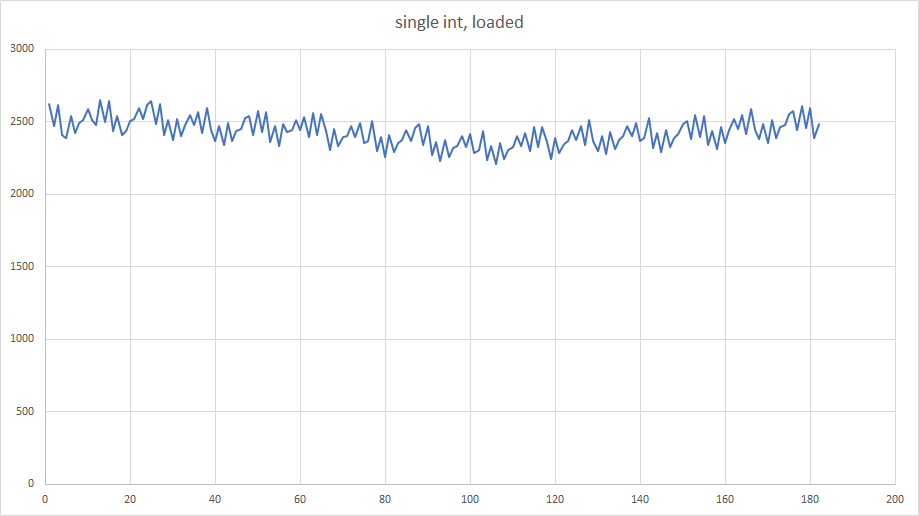
\includegraphics[width=0.75\textwidth]{Project3ControllerStateMachine/rpm_distortions.png}
    \caption{repeating pattern indicating inaccuracies in the encoder wheel}
    \label{fig:distortedRpm}
\end{figure}
\\
The rpm was stabilized further by taking a rolling average of the measured values and it was determined that the average of 10 samples would be adequate to reach a clean waveform.
%However, delaying the input to the pi controller for 50ms may result in the system becoming unstable since the controller might overcompensate for the error if it doesn't see the change it's trying to make have any immediate effect resulting in oscillations. A possible solution would be to decrease the time between cycles or shorten the averaging period
\\
\section{Part 4}


%\subsection{Tuning the system} 

\begin{figure}[H]
    \centering
    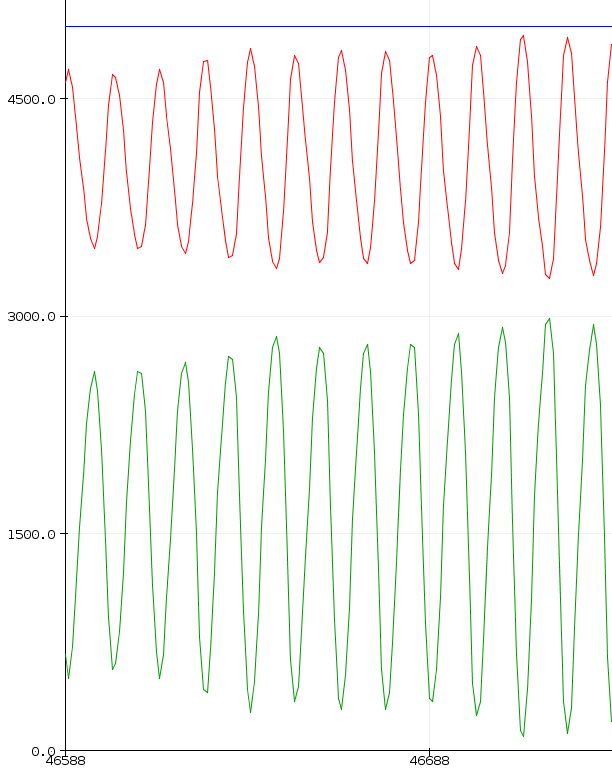
\includegraphics[width=0.75\textwidth]{Project3ControllerStateMachine/oscillate_p72.png}
    \caption{Stable Oscillations were observed with \(K_p = 7.2, K_i=0\), Set point is in blue, the observed rpm is in red and the scaled up pwm duty is in green}
    \label{fig:oscillations}
\end{figure}

The Ziegler-Nichols method was used to tune the system. The integral gain was set to zero and proportional gain was increased until stable  oscillations could be seen in the output. A graph of the oscillations can be seen in Figure \ref{fig:oscillations}. The ultimate gain was found to be \(K_u = 7.2\), \(T_u = 26 ms\), At that point a suitable values for \(K_p\) and \(K_i\) were fetched from a table according to the Ziegler-Nichols tuning method giving \(K_p=3.45\) and  \(K_i=150\)
\\

With the new values the system behaved quite nicely as can be seen in the step response in Figure \ref{fig:stepResponse}

A good load reponse pattern may be seen in figure \ref{fig:LoadResponse}


\begin{figure}[H]
    \centering
    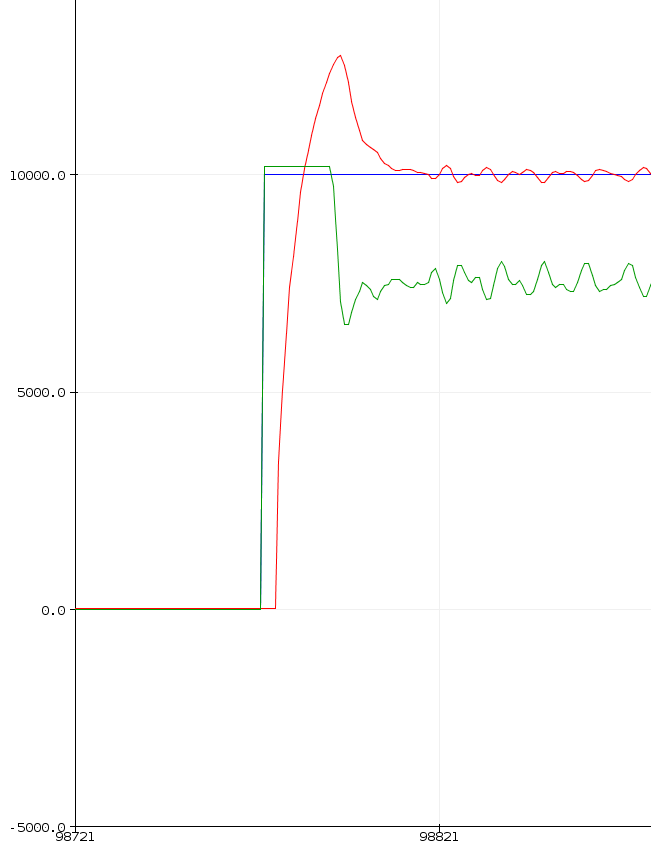
\includegraphics[width=0.75\textwidth]{Project3ControllerStateMachine/Step_p324_i120.png}
    \caption{step response from 0 to 10krpm with  \(K_p = 3.24, K_i=150\), Set point is in blue, the observed rpm is in red and the scaled up pwm duty is in green}
    \label{fig:stepResponse}
\end{figure}

%Determining when oscillations were of suitable amplitude proved difficult since there was a non-insignificant instability in the rpm signal and therefore constant oscillations. 
\\
\\
With the new rpm method counting the pulses of the rotary encoder is strictly unnecessary but it was necessary to monitor both phases to determine which direction the motor was turning. Having the counts could also help for future use. 

%\subsection{Step  and load response}
\begin{figure}[H]
    \centering
    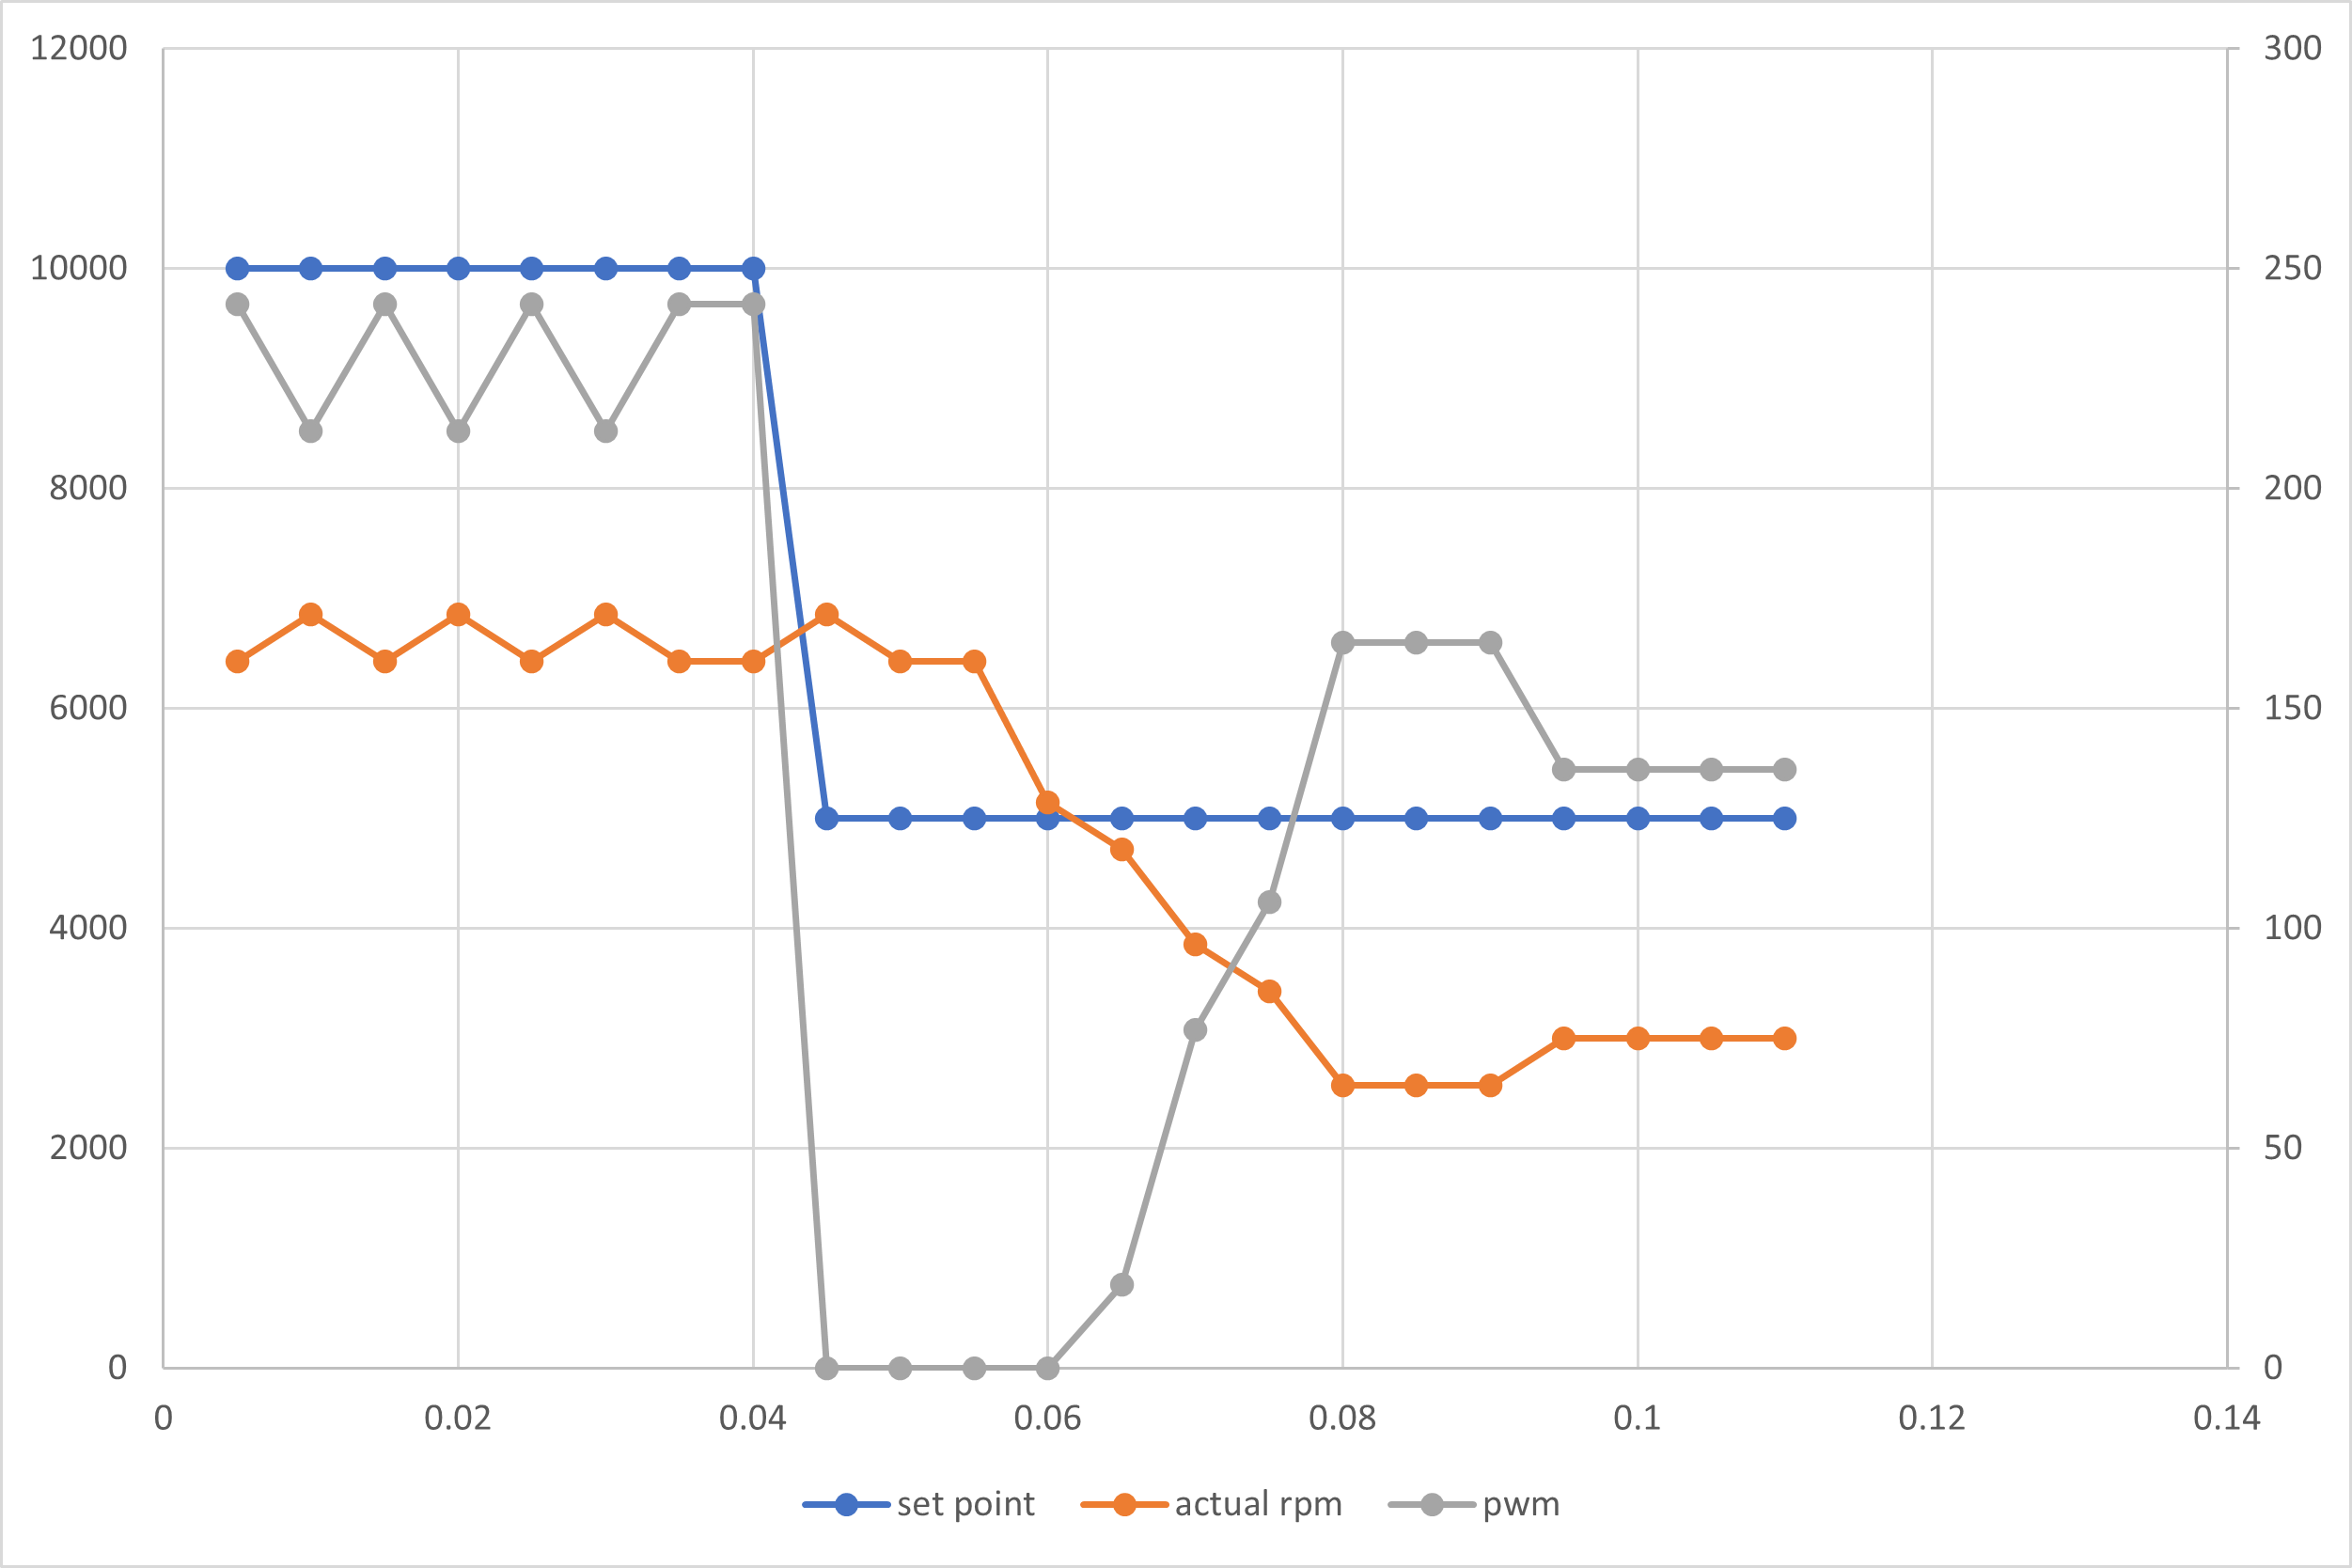
\includegraphics[width=0.75\textwidth]{Project2SpeedController/step_response2.png}
    \caption{Step response for old p controller}
    \label{fig:oldStepResponse}
\end{figure}

\begin{figure}[H]
    \centering
    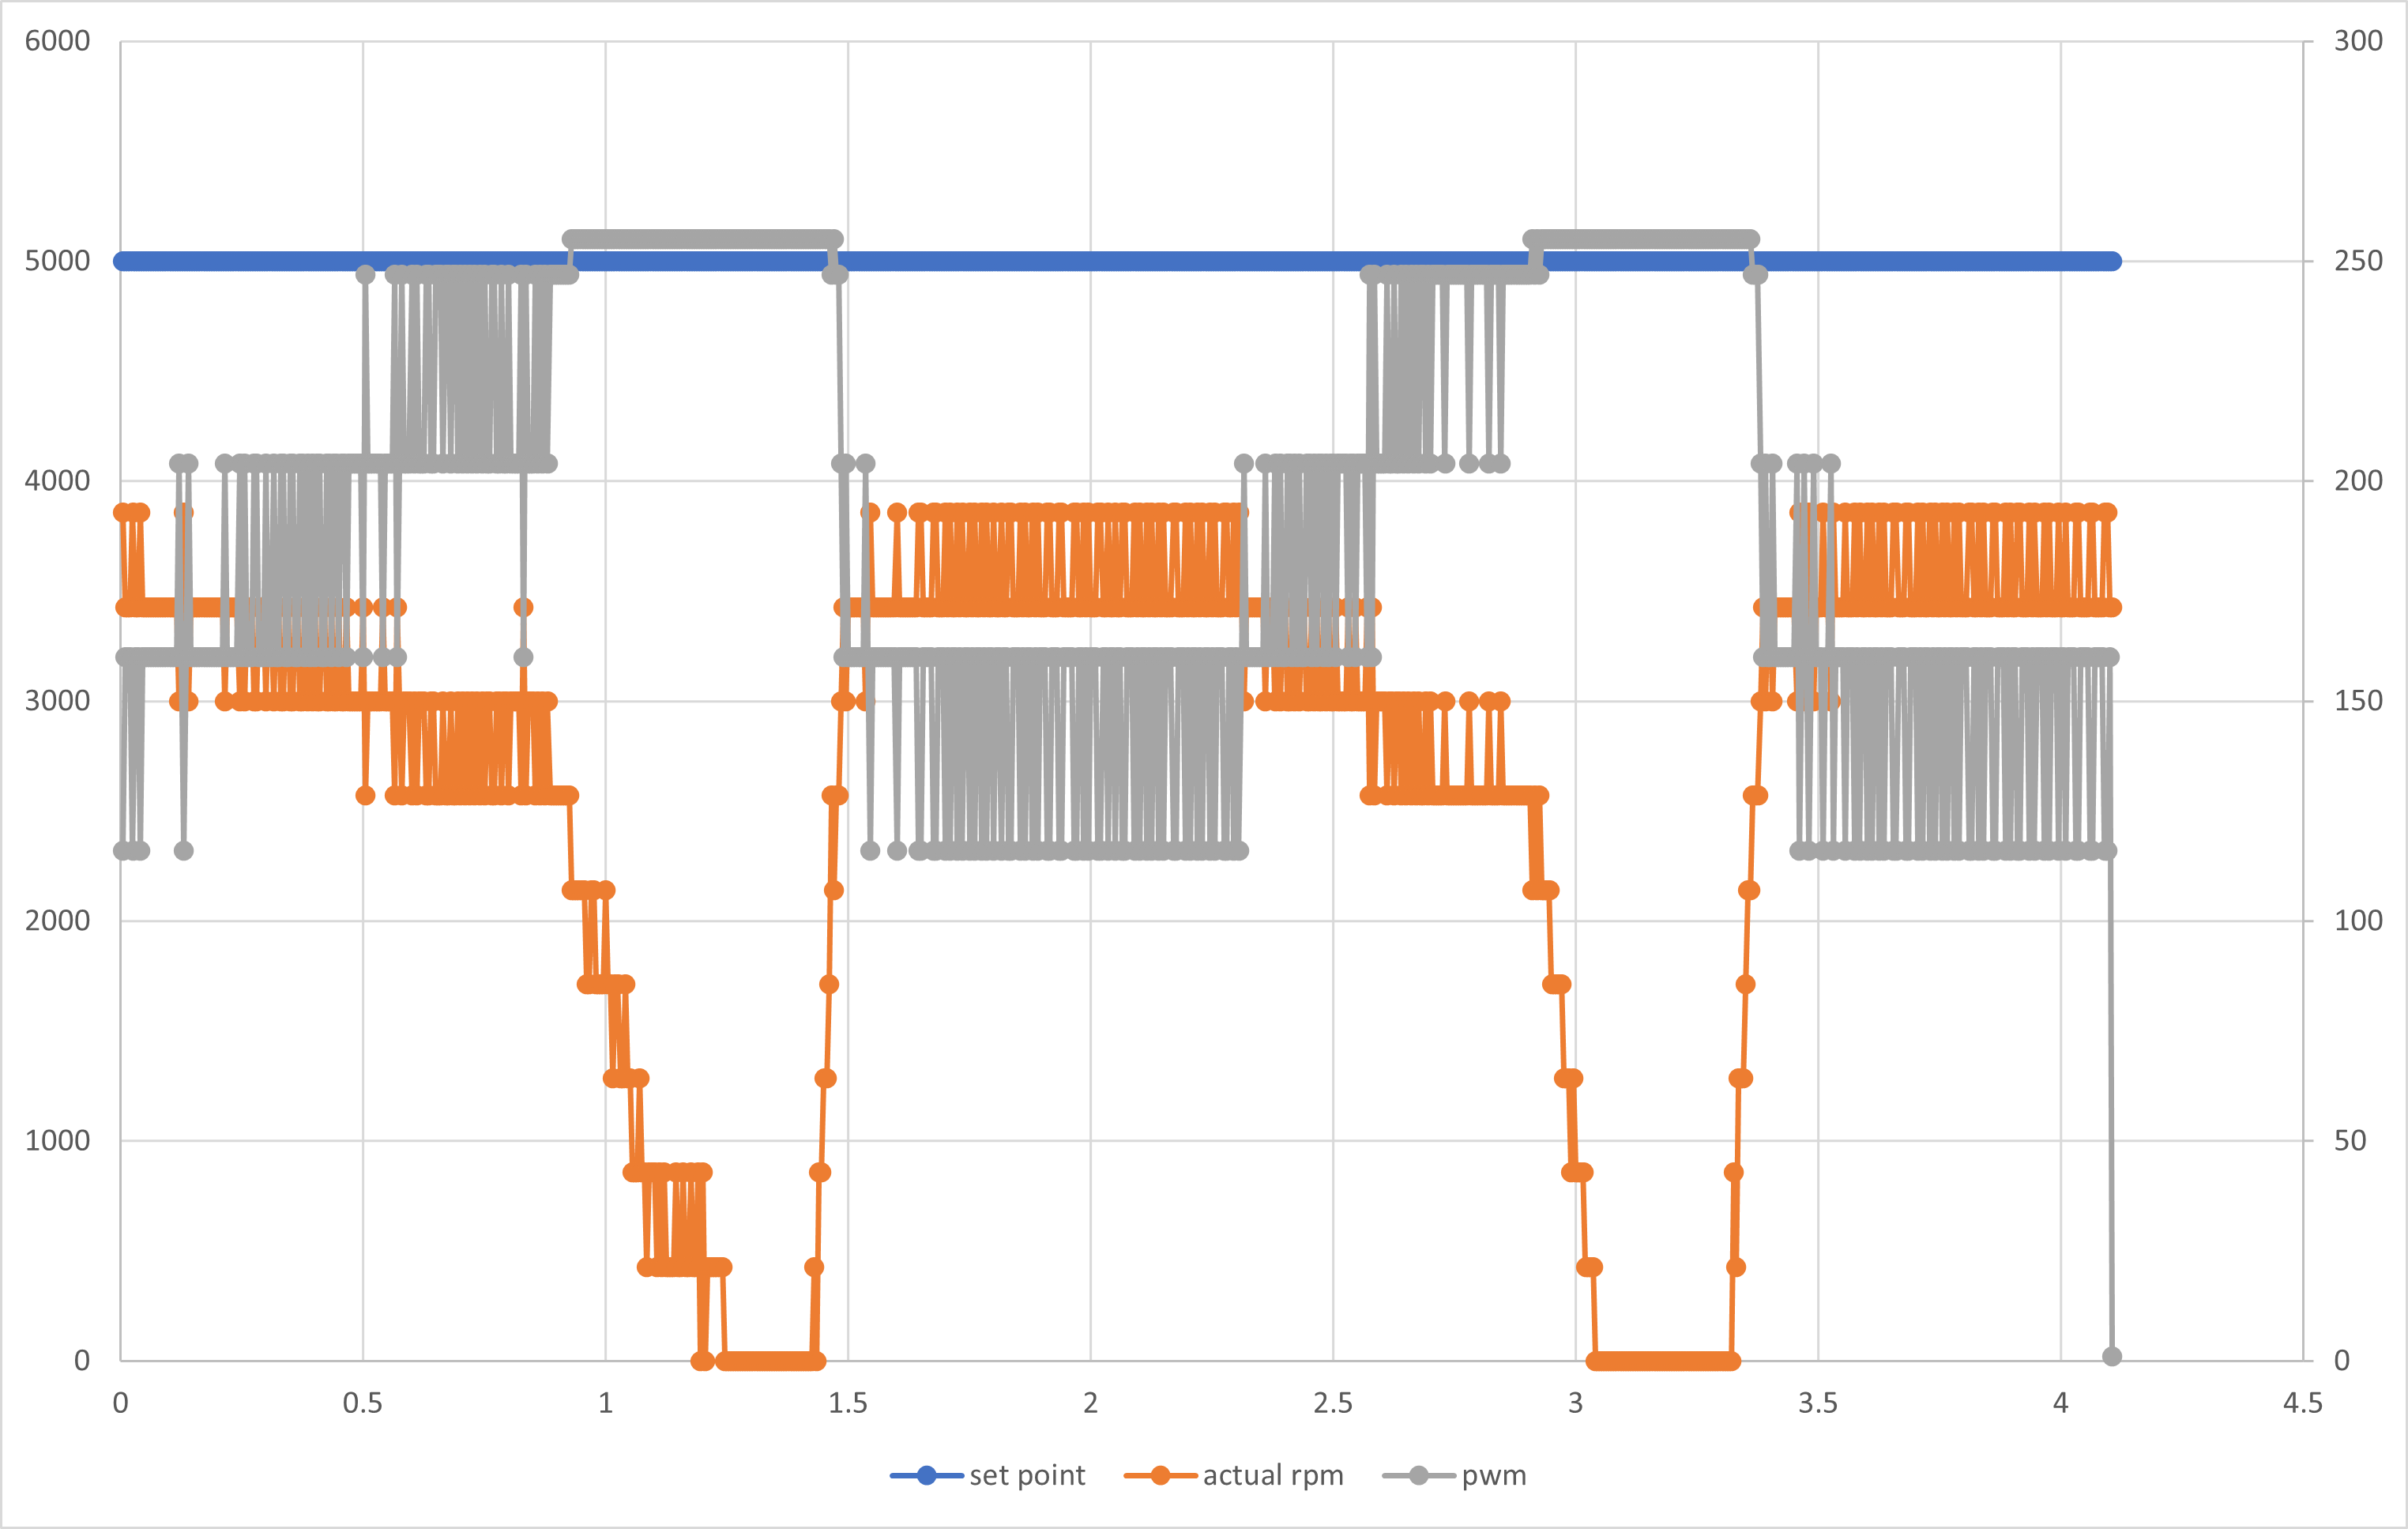
\includegraphics[width=0.75\textwidth]{Project2SpeedController/load_response.png}
    \caption{load response for old p controller}
    \label{fig:oldLoadResponse}
\end{figure}

\begin{figure}[H]
    \centering
    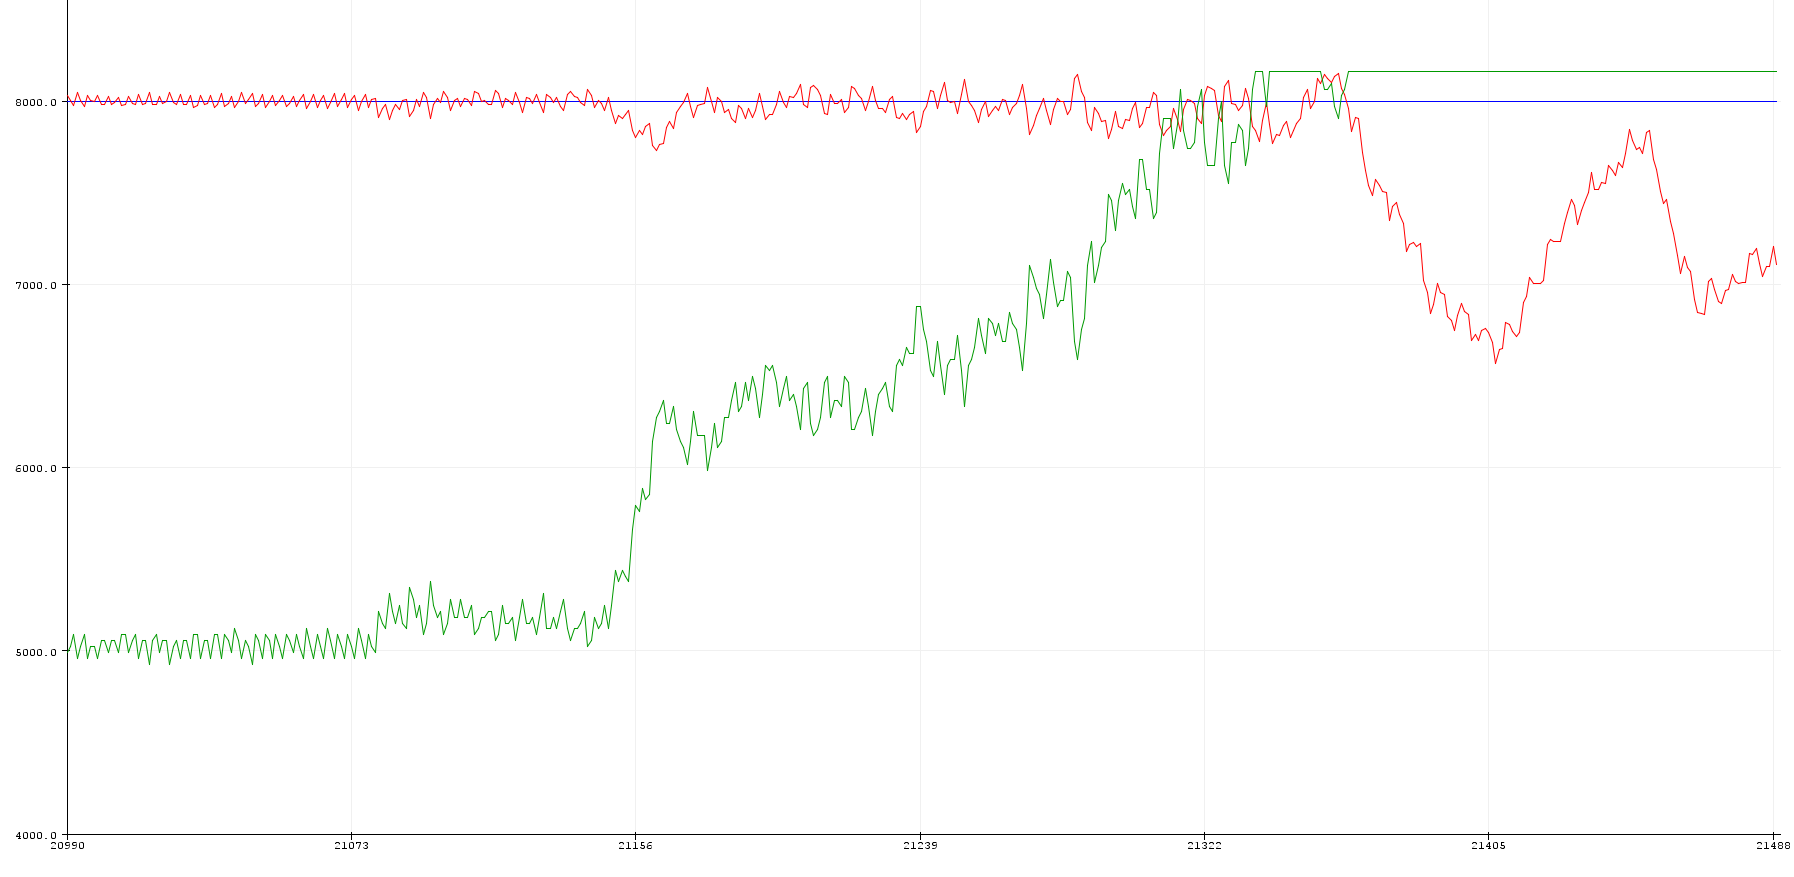
\includegraphics[width=0.75\textwidth]{Project3ControllerStateMachine/load_response.png}
    \caption{load response for the new PI controller. Set point is in blue, the observed rpm is in red and the scaled up pwm duty is in green}
    \label{fig:LoadResponse}
\end{figure}


\ 
\newpage
A video showing the motor controller in operation can be seen at \url{https://youtu.be/YvaofKchtCM}
The code used can be found on github at \url{https://github.com/Steinarr134/EmbeddedGroupProjects/tree/main/Project3ControllerStateMachine} 
\section{Discussion}

Initially, there were problems with timer0 and timer1. 
\\
Timer0 wouldn't set a compare match interrupt until TCNT0 register was manually set to 0 in the interrupt routine. Additionally, timer0 would get glitched and not interrupt at the correct period rather interrupt at delta\_t plus time. This proved to happen exclusively when timer1 overflow interrupt ran, however, the timer1 overflow interrupt wasn't being used so disabling it ameliorated the issue.
\\
The encoder on the motor seems to be rather poorly made, the position of the magnetic sensors is not controlled accurately which causes the pulse width, between phases, at a constant rpm, to be inconsistent. Too inconsistent for it to be able to use the separate phases for higher resolution in rpm values. Although, 14 pulses per revolution is very adequate and it's certainly better than the previous method to measure rpm and the previous method seemed to be good enough. 
\section*{Appendix}
\appendix

\newpage
\section{Code}\label{appendix:code}

\lstinputlisting[caption=main program used to produce the step response]{Project2SpeedController/src/main.cpp}

\lstinputlisting[caption=timer\_msec.cpp]{Project1RotaryEncoder/src/encoder_simple.cpp}

\lstinputlisting[caption=main.cpp]{Project1RotaryEncoder/src/main.cpp}

\end{document}
